\documentclass{beamer}

\usepackage[utf8]{inputenc}

\usepackage{color}
\usepackage{listings}
\usepackage{tikz}
\usepackage{hyperref}

\usetheme{Rochester}
\usecolortheme{beaver}

\lstloadlanguages{[5.2]Lua,C++}
    \lstset{%
        language={[5.2]Lua},
        basicstyle=\ttfamily,
        keywordstyle=\color{blue},
        showstringspaces=false,
        escapechar={§},
        escapeinside=||
    }

\newif\iftransitions
% \transitionstrue


\title{Howling at the Moon:}
\subtitle{Lua for C++ Programmers}
\author{Andreas Weis}
\institute{BMW AG}
\date{cppcon, September 29, 2017}
\titlegraphic{
\includegraphics[height=.25\textheight]{resources/cppcon.png}}


\begin{document}

\frame{\titlepage}

\begin{frame}[fragile]
  \frametitle{About me}

  \begin{itemize}
    \setlength\itemsep{1.5em}

    \item \href{https://stackoverflow.com/users/577603/comicsansms}{
\includegraphics[height=.05\textheight]{resources/so-icon.png}} \href{https://github.com/ComicSansMS}{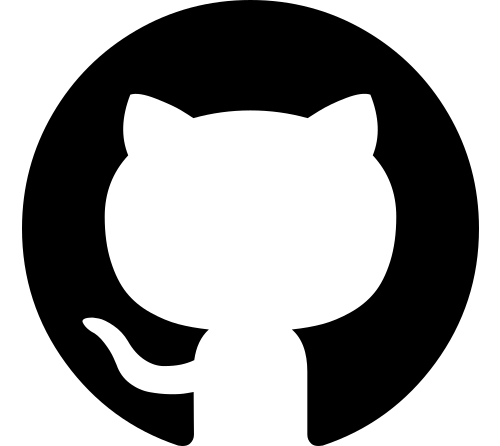
\includegraphics[height=.05\textheight]{resources/github-icon.png}} 
\includegraphics[height=.05\textheight]{resources/slack-icon.png} Known as ComicSansMS on most sites

    \item \href{https://twitter.com/DerGhulbus/}{
\includegraphics[height=.05\textheight]{resources/twitter-icon.png} @DerGhulbus on Twitter}

    \item 
\includegraphics[height=.05\textheight]{resources/meetup-icon.png} Co-organizer of the \href{https://www.meetup.com/MUCplusplus/}{Munich C++ User Group}

    \item Currently working as a Software Architect for BMW 
\includegraphics[height=.1\textheight]{resources/bmw_group.jpg}

  \end{itemize}
\end{frame}

\begin{frame}[fragile]

  \begin{center}
    \href{http://www.lua.org/}{
\includegraphics[height=.8\textheight]{resources/lua-logo.png}}
  \end{center}

\end{frame}

\begin{frame}[fragile]
  \frametitle{Lua}

  \begin{quote}Lua is a powerful, efficient, lightweight, embeddable scripting language.\end{quote}

  \pause

  \begin{itemize}
    \item Powerful
    \item Efficient
    \item Lightweight
    \item Embeddable
  \end{itemize}

  \begin{itemize}
  \item Powerful - First-class functions w/ full lexical scoping; Support for OOP paradigms; Metaprogramming; Reflection
  \item Efficient - Performance better or on par with other scripting languages; Even better with LuaJIT
  \item Lightweight - Small binaries; Only one type of complex data structure; Great expressiveness through few, orthogonal constructs
  \item Embeddable - Simple and lean API; \texttt{main()} belongs to the enclosing program
  \end{itemize}

\end{frame}

\begin{frame}
  \frametitle{Use cases}

  @todo Images

  \begin{itemize}
  \item Games (Lua Bar, World of Warcraft)
  \item Adobe Lightroom
  \item Embedded (NodeMCU)
  \end{itemize}
\end{frame}

\begin{frame}
  \frametitle{Why bother with Lua?}

  Lua is \emph{small}.

  (In a good way)

  The interpreter fits into L2 cache of a modern desktop x86.

  \begin{itemize}
  \item The whole language fits in your head.
  \item No swapping required.
  \end{itemize}
\end{frame}

\begin{frame}[fragile]
  \frametitle{Hello World!}

  \begin{lstlisting}
print("Hello World!");
  \end{lstlisting}
\end{frame}

\begin{frame}[fragile]

  \frametitle{Functions}

  \begin{lstlisting}
function f(a1, a2, a3)
  -- implementation
  -- [...]
  return r1, r2, r3;
end


y1, y2, y3 = f(x1, x2, x3);
y1 = f(x1, x2, x3);
f();
  \end{lstlisting}

\end{frame}

\begin{frame}[fragile]
  \frametitle{All functions are lambdas}

  \begin{lstlisting}
f = function(a1, a2, a3)
  -- implementation
  -- [...]
  return r1, r2, r3;
end
  \end{lstlisting}

  Functions are true first-class values in Lua.
\end{frame}

\begin{frame}[fragile]
  \frametitle{Replacing functions is trivial}

  \begin{lstlisting}
print("Vanilla print");
print = function(...)
    -- my_print implementation
  end;
print("My print");
  \end{lstlisting}
\end{frame}

\begin{frame}[fragile]

  \frametitle{Counting \texttt{print} calls}

  Instead of explicit Lambda captures, Lua has full lexical scoping.

  \begin{lstlisting}
count = 0;
old_print = print;
print = function(...)
    count = count + 1;
    old_print(...);
  end;
  \end{lstlisting}

\end{frame}


\begin{frame}[fragile]

  \frametitle{Capturing state with function closures}

  Instead of explicit Lambda captures, Lua has full lexical scoping.

  \begin{lstlisting}
function enable_counting()
  local count = 0;
  local old_print = print;
  print = function(...)
      count = count + 1;
      old_print(...);
    end;

  return function() return count; end;
end
  \end{lstlisting}

  Read \texttt{function} as closure construction.
\end{frame}


\begin{frame}[fragile]
  \frametitle{Tables}

  The only complex data structure in the language.

  \begin{lstlisting}
local t = {};

local array = { 5, 4, 3, 2, 1 };
assert(array[2] == 3);   -- indices are 1-based

local dict = { the_answer = 42 };
assert(dict["the_answer"] == 42);
  \end{lstlisting}

  Tables can use any type of values as keys or values.

  \begin{lstlisting}
dict[print] = "function as key";
  \end{lstlisting}

  Read \texttt{\{\}} as table construction.
\end{frame}

\begin{frame}[fragile]

  \frametitle{Records}

  \begin{lstlisting}
local complex = { real = 42.0, imag = 0.0 };

function conjugate(c)
  c.imag = 0.0 - c.imag;
end
  \end{lstlisting}

  Tables have reference semantics.

  Table equality is pointer identity.

  \begin{lstlisting}
complex.conjugate = conjugate;
complex.conjugate(complex)
complex:conjugate();
  \end{lstlisting}

\end{frame}

\begin{frame}[fragile]
  \frametitle{Object Construction}

  \begin{lstlisting}
function build_complex(r, i)
  return { real = r, imag = i };
end

local c1 = build_complex(1, 0);
local c2 = build_complex(0, 1);
  \end{lstlisting}

  \begin{lstlisting}
local sum = c1 + c2; -- ???
  \end{lstlisting}
\end{frame}


\begin{frame}[fragile]
  \frametitle{Metatables - Tables describing object properties}

  \begin{lstlisting}
function build_complex(r,i)
  local mt = {};
  mt.__add = function(c1, c2)
    return build_complex(c1.real + c2.real,
    c1.imag + c2.imag);
    end;
    local ret = {}
  \end{lstlisting}
\end{frame}


\begin{frame}[fragile]
  \frametitle{Metatables on non-table values}

  \begin{lstlisting}
local str = "The quick brown fox";
assert(str:find("quick") == 5)
  \end{lstlisting}

  Metatables are extensible: Functions can add their own semantics for non-standard fields.
\end{frame}


\iftransitions

\begin{frame}[fragile]
  \frametitle{Encapsulation}
  \setbeamercolor{alerted text}{fg=red}
  \setbeamerfont{alerted text}{series=\bfseries,family=\ttfamily}
  \begin{semiverbatim}
\uncover<1->{\alert<0>{{\color{blue}function} newDate(y, m, d)}}
\uncover<3->{\alert<3>{  assert(validDate(y, m, d))}}
\uncover<3->{\alert<3>{  {\color{blue}local} self = \{ y=y, m=m, d=d \}}}
\uncover<3->{\alert<3>{}}
\uncover<4->{\alert<4>{  {\color{blue}local} getDay = {\color{blue}function}() {\color{blue}return} self.d {\color{blue}end}}}
\uncover<5->{\alert<5>{  {\color{blue}local} setDay = {\color{blue}function}(nd)}}
\uncover<5->{\alert<5>{      assert(validDate(self.y, self.m, nd))}}
\uncover<5->{\alert<5>{      self.d = nd}}
\uncover<5->{\alert<5>{    {\color{blue}end}}}
\uncover<5->{\alert<5>{}}
\uncover<2->{\alert<2>{  {\color{blue}return} \{}}
\uncover<2->{\alert<2>{    setDay = setDay,}}
\uncover<2->{\alert<2>{    getDay = getDay}}
\uncover<2->{\alert<2>{  \}}}
\uncover<1->{\alert<0>{\color{blue}end}}
  \end{semiverbatim}
\uncover<6->{}
\end{frame}

\else

\begin{frame}[fragile]
  \frametitle{Encapsulation}

  \begin{lstlisting}
function newDate(y, m, d)
  assert(validDate(y, m, d))
  local self = { y=y, m=m, d=d }

  local getDay = function() return self.d end
  local setDay = function(nd)
      assert(validDate(self.y, self.m, nd))
      self.d = nd
    end

  return {
    setDay = setDay,
    getDay = getDay
  }
  \end{lstlisting}
\end{frame}

\fi


\begin{frame}[fragile]
  \frametitle{Reflection}

  All data structures are tables. Inspecting the fields of the table reveals everything we need to know.

  \begin{lstlisting}
function is_complex(c)
  return c.real and c.imag;    
end
  \end{lstlisting}

  \begin{lstlisting}
local tuple = {};
for k,v in pairs(t) do
  tuple[#tuple + 1] = v;
end
  \end{lstlisting}
\end{frame}


\begin{frame}[fragile]

  \frametitle{The environment}

  But what about global variables?

  \begin{lstlisting}
for k in pairs(_G) do
  print(k);
end
  \end{lstlisting}

  What about local variables?
  Sorry, no.
\end{frame}


\begin{frame}[fragile]

  \frametitle{Constraining the environment}

  \begin{lstlisting}
local foobar;
-- [...]
fobar = do_stuff();
  \end{lstlisting}

  \texttt{\_G} is just a table.

  \begin{lstlisting}
setmetatable(_G, {__newindex = function() print("No!"); end});
  \end{lstlisting}
  
\end{frame}


\frame{%
\setbeamercolor{normal text}{fg=gray,bg=}
\setbeamercolor{alerted text}{fg=black,bg=}
\usebeamercolor{normal text}
\begin{itemize}
\item \alert<+>{Hallo}
\item \alert<+>{Welt}
\item \alert<+>{Foobar}
\end{itemize}
}


\iffalse

\begin{frame}[fragile]
    \frametitle{Outline}
    \begin{itemize}
        \item This talk tries to focus on the big features.
        \item We will not discuss C++17 only, but also some of the features that are currently specified as a TS.
        \item Still, there's lots of stuff that we won't talk about.
        \item For a complete list of what's new in C++17, check out Alisdair Meredith's CppCon talk \emph{C++17 in Breadth (Not Depth)}\footnote{\url{https://www.youtube.com/watch?v=22jIHfvelZk}}
        \item Feel free to disagree on whether the features discussed here will have a major impact.
    \end{itemize}
\end{frame}

\iffalse
\begin{frame}
  \frametitle{What we wanted}
  \begin{itemize}
    \item Concepts
    \item Modules
    \item Ranges
    \item Networking
    \item Coroutines
    \item Uniform Call Syntax
    \item Contracts
    \item Vocabulary Types (optional, variant)

    \item SIMD and parallel algorithms
    \item \texttt{stack\_array}
  \end{itemize}
\end{frame}

\begin{frame}
  \frametitle{What we got}
  \begin{itemize}
    \item Structured bindings
    \item \texttt{if} and \texttt{switch} with initializer
    \item \texttt{if constexpr}
  \end{itemize}
\end{frame}
\fi


\begin{frame}[fragile]
  \frametitle{\texttt{if constexpr}}
    \begin{itemize}
      \item Basically a smarter \texttt{\#if}
      \item Goes back to proposal N3329 from 2012, heavily inspired by D's \texttt{static if} (introduced there in 2005)\footnote{see also Alexandrescu's Going Native 2012 talk \emph{Static if I had a hammer}}
      \item Was held back because of concerns about overlap with Concepts and uncertainty about scoping
      \item Re-proposed as \texttt{if constexpr} in 2016 (after Concepts Lite), with slightly different semantics
    \end{itemize}
\end{frame}


\begin{frame}[fragile]
  \frametitle{Compile time branching is weird}
    \begin{lstlisting}[language=C++,basicstyle=\ttfamily,keywordstyle=\color{blue},showstringspaces=false]
template<class T>
struct is_awesome;

template<class T>
void compute_stuff()
{
  if(is_awesome<T>::value) {
    // awesome algorithm
    // ...
  } else {
    // slightly less awesome algorithm
    // ...
  }
}
    \end{lstlisting}
\end{frame}


\begin{frame}[fragile]
  \frametitle{Compile time branching is weird}
    \begin{itemize}
        \item Compiler will (insistently) warn that you are branching on a compile-time constant condition.
        \item Both branches need to compile for all valid \texttt{T}s.
        \item Runtime branching does not cut it. What we really want is \emph{conditional compilation}.
    \end{itemize}
\end{frame}


\begin{frame}[fragile]
  \frametitle{SFINAE to the rescue!}
    \begin{lstlisting}[language=C++,basicstyle=\ttfamily,keywordstyle=\color{blue},showstringspaces=false]
template<class T>
std::enable_if_t<is_awesome<T>::value>
  compute_stuff()
{
  // awesome algorithm
  // ...
}

template<class T>
std::enable_if_t<!is_awesome<T>::value>
  compute_stuff()
{
  // slightly less awesome algorithm
  // ...
}
    \end{lstlisting}
\end{frame}


\begin{frame}[fragile]
  \frametitle{SFINAE to the rescue?}
    \begin{itemize}
        \item Lots of boilerplate and code duplication.
        \item Requires intimate knowledge of what many consider a weird corner case of C++ templates.
        \item \texttt{std::enable\_if} makes stuff easier, but is still prone to breaking in non-obious ways.
\iffalse        \item No compile time manipulation of state and layout (replace method with \texttt{static} member) \fi
    \end{itemize}
\end{frame}


\begin{frame}[fragile]
  \frametitle{\texttt{if constexpr}}
    \begin{lstlisting}[language=C++,basicstyle=\ttfamily,keywordstyle=\color{blue},showstringspaces=false]
template<class T>
void compute_stuff()
{
  if constexpr(is_awesome<T>::value) {
    // awesome algorithm
    // ...
  } else {
    // slightly less awesome algorithm
    // ...
  }
}
    \end{lstlisting}
    The discarded branch is not instantiated by the compiler. Otherwise behaves like a regular \texttt{if} statement.
\end{frame}


\begin{frame}
  \frametitle{\texttt{if constexpr}}
    \begin{itemize}
        \item This is less powerful than the initial \texttt{static if} idea,
              which was much closer to \texttt{\#if} than to \texttt{if}.
        \item No branching at global or namespace scope.
        \item No layout changes.
        \item \texttt{if constexpr} introduces new scope.
    \end{itemize}
\end{frame}


\begin{frame}[fragile]
  \frametitle{Compiler support for if constexpr}
    Only gcc 7 and clang 3.9 support it already.
\end{frame}


\begin{frame}[fragile]
  \frametitle{\texttt{if} and \texttt{switch} with initializer}
    \begin{lstlisting}[language=C++,basicstyle=\ttfamily,keywordstyle=\color{blue},showstringspaces=false]
void safe_init() {
  {
    std::lock_guard<std::mutex> lk(mx_);
    if(v.empty()) {
      v.push_back(kInitialValue);
    }
  }
  // ...
}
    \end{lstlisting}
    \begin{itemize}
        \item Need an additional pair of \texttt{\{\}}s for scoping lock
        \item When refactoring, take care that the \texttt{if} cannot be separated from the lock
    \end{itemize}
\end{frame}


\begin{frame}[fragile]
  \frametitle{\texttt{if} and \texttt{switch} with initializer}
    \begin{lstlisting}[language=C++,basicstyle=\ttfamily,keywordstyle=\color{blue},showstringspaces=false]
void safe_init() {
  if(std::lock_guard<std::mutex> lk(mx_);
      v.empty()) {
    v.push_back(kInitialValue);
  }
  // ...
}
    \end{lstlisting}
    \begin{itemize}
        \item \texttt{lk} is scoped by the \texttt{if}.
    \end{itemize}
\end{frame}


\begin{frame}[fragile]
  \frametitle{\texttt{if} and \texttt{switch} with initializer}
    \begin{lstlisting}[language=C++,basicstyle=\ttfamily,keywordstyle=\color{blue},showstringspaces=false]
if(auto p = m.try_emplace(key, value);
   !p.second)
{
  FATAL("Element already registered");
} else {
  process(p.second);
}
    \end{lstlisting}
    \begin{itemize}
        \item Avoids polluting the enclosing namespace with identifiers.
    \end{itemize}
\end{frame}


\begin{frame}[fragile]
  \frametitle{Compiler support for \texttt{if} and \texttt{switch} with initializer}
    Only gcc 7 and clang 3.9 support it already.
\end{frame}


\begin{frame}[fragile]
  \frametitle{Structured Bindings}
  \texttt{std::tie} is not as useful as it should be:
    \begin{lstlisting}[language=C++,basicstyle=\ttfamily,keywordstyle=\color{blue},showstringspaces=false]
std::map<std::string, int> my_map;
auto const ret = my_map.insert({"key", 42});

std::map<std::string, int>::iterator it;
bool was_inserted;
std::tie(it, was_inserted) = ret;

    \end{lstlisting}
    \begin{itemize}
        \item We lose type deduction for the iterator type.
        \item We lose the const qualifier.
        \item Separate declaration often not feasible for non-trivial types.
    \end{itemize}
\end{frame}


\begin{frame}[fragile]
  \frametitle{Structured Bindings - To the rescue!}
    \begin{lstlisting}[language=C++,basicstyle=\ttfamily,keywordstyle=\color{blue},showstringspaces=false]
std::map<std::string, int> my_map;

auto const [it, was_inserted] =
    my_map.insert({"key", 42});
    \end{lstlisting}
\end{frame}


\begin{frame}[fragile]
  \frametitle{Structured Bindings - Destructuring}
    But wait, there's more:
    \begin{lstlisting}[language=C++,basicstyle=\ttfamily,keywordstyle=\color{blue},showstringspaces=false]
struct Foo {
    int i;
    float f;
    std::string s;
};

Foo f;
// ...
auto [natural, real, text] = f;
    \end{lstlisting}
\end{frame}


\begin{frame}[fragile]
  \frametitle{Structured Bindings}
  Alright, cool. But how is this a major feature?
\end{frame}


\begin{frame}[fragile]
  \frametitle{Some preliminary boilerplate...}
    \begin{lstlisting}[language=C++,basicstyle=\ttfamily,keywordstyle=\color{blue},showstringspaces=false]
struct any_type {
  template<class T>
  constexpr operator T(); // non explicit
};
    \end{lstlisting}

    \begin{lstlisting}[language=C++,basicstyle=\ttfamily,keywordstyle=\color{blue},showstringspaces=false]
template <class T, class... TArgs>
class is_braces_constructible;
  // std::true_type if we can construct
  // a T from the TArgs
    \end{lstlisting}
\end{frame}


\begin{frame}[fragile]
  \frametitle{Struct to tuple}
    \begin{lstlisting}[language=C++,basicstyle=\ttfamily,keywordstyle=\color{blue},showstringspaces=false]
template<class T> auto to_tuple(T&& object) {
  using type = std::decay_t<T>;
  if constexpr(is_braces_constructible
          <type, any_type, any_type>{})
  {
    auto&& [p1, p2] = object;
    return std::make_tuple(p1, p2);
  } else if constexpr(is_braces_constructible
          <type, any_type>{})
  {
    auto&& [p1] = object;
    return std::make_tuple(p1);
  } else {
    return std::make_tuple();
  }
}
    \end{lstlisting}
\end{frame}


\begin{frame}
  \frametitle{Simple compile-time reflection}

    Full example at \url{https://www.reddit.com/r/cpp/comments/4yp7fv/c17_structured_bindings_convert_struct_to_a_tuple/}.

    \begin{itemize}
        \item Once we have tuples, we can do all kinds of metaprogramming (see Boost Hana)
        \item Not clear how much benefit structured bindings really bring, but chances are they will turn out more powerful than they seem at first glance.
    \end{itemize}
\end{frame}


\begin{frame}[fragile]
    \frametitle{Structured bindings + \texttt{if} with initializer}
    \begin{lstlisting}[language=C++,basicstyle=\ttfamily,keywordstyle=\color{blue},showstringspaces=false]
std::map<std::string, int> my_map;
if(auto const [it, was_inserted] = 
        my_map.insert({"key", 42});
   !was_inserted)
{
    throw InsertionFailed();
}
    \end{lstlisting}
\end{frame}

\begin{frame}
    \frametitle{Compiler support for structured bindings}

    Only (partially) supported in Clang 4.0 today.
\end{frame}


\begin{frame}[fragile]
  \frametitle{Concepts TS (not part of C++17)}
    Specify constraints for template arguments.
    \begin{lstlisting}[language=C++,basicstyle=\ttfamily,keywordstyle=\color{blue},showstringspaces=false]
template<typename T>
T const& min(T const& a, T const& b)
{
    return (a < b) ? a : b;
}
    \end{lstlisting}
\end{frame}


\begin{frame}[fragile]
  \frametitle{Concepts Example}
    \begin{lstlisting}[language=C++,basicstyle=\ttfamily,keywordstyle=\color{blue},showstringspaces=false]
template<typename T>
concept bool LTComparable = requires(T a, T b)
{
    { a < b } -> bool;    
};

template<LTComparable T>
T const& min(T const& a, T const& b)
{
    return (a < b) ? a : b;
}
    \end{lstlisting}
\end{frame}

\begin{frame}[fragile]
  \frametitle{Error messages with concepts}
  Here's what happens if we try to use \texttt{min} with a type \texttt{Foo} that does not have \texttt{operator<}:
  \tiny {
    \begin{lstlisting}[basicstyle=\ttfamily]
In function 'int main()':
error: cannot call function 'const T& min(const T&, const T&) [with T = Foo]'
   std::cout << min(a, b) << std::endl;
                        ^
note:   constraints not satisfied
 T const& min(T const& a, T const& b)
          ^~~
note: within 'template<class T> concept const bool LTComparable<T> [with T = Foo]'
 concept bool LTComparable = requires(T a, T b) {
              ^~~~~~~~~~~~
note:     with 'Foo a'
note:     with 'Foo b'
note: the required expression '(a < b)' would be ill-formed
    \end{lstlisting}
  }
\end{frame}


\begin{frame}[fragile]
  \frametitle{Error messages with concepts}
  Here's what happens if there is an \texttt{operator<}, but it does not return \texttt{bool}:
  \tiny {
    \begin{lstlisting}[basicstyle=\ttfamily]
In function 'int main()':
error: cannot call function 'const T& min(const T&, const T&) [with T = Foo]'
   std::cout << min(a, b) << std::endl;
                        ^
note:   constraints not satisfied
 T const& min(T const& a, T const& b)
          ^~~
note: within 'template<class T> concept const bool LTComparable<T> [with T = Foo]'
 concept bool LTComparable = requires(T a, T b) {
              ^~~~~~~~~~~~
note:     with 'Foo a'
note:     with 'Foo b'
note: 'operator<(a, b)' is not implicitly convertible to 'bool'
    \end{lstlisting}
  }
\end{frame}


\begin{frame}[fragile]
    \begin{itemize}
    \frametitle{Concepts}
    \item Concepts are not checked for completeness. The implementation may use a concept parameter like any \texttt{typename}.
    \begin{lstlisting}[language=C++,basicstyle=\ttfamily,keywordstyle=\color{blue},showstringspaces=false]
template<LTComparable T>
T const& max(T const& a, T const& b)
{
    return (a > b) ? a : b;
}
    \end{lstlisting}
    \item Constraints can be used instead of SFINAE to remove functions from the overload set.
    \begin{lstlisting}[language=C++,basicstyle=\ttfamily,keywordstyle=\color{blue},showstringspaces=false]
template<typename T>
requires std::is_integral<T>::value
void ints_only(T i);
    \end{lstlisting}
    \end{itemize}
\end{frame}


\begin{frame}[fragile]
  \frametitle{Writing concepts}
  \begin{quote}Defining good concepts is non-trivial. Concepts are meant to represent fundamental concepts in an application domain (hence the name "concepts"). Similarly throwing together a set of syntactic constraints to be used for a the arguments for a single class or algorithm is not what concepts were designed for and will not give the full benefits of the mechanism.\end{quote}
  
  From the C++ Core Guidelines \footnote{\url{https://github.com/isocpp/CppCoreGuidelines/blob/master/CppCoreGuidelines.md\#t20-avoid-concepts-without-meaningful-semantics}}
\end{frame}


\begin{frame}[fragile]
  \frametitle{Writing concepts}
  \begin{itemize}
    \item In the current TS, concepts only allow checking syntactical properties.
    \item However, concepts should only be designed from meaningful semantics (potentially including space/time complexity).
    \item Unfortunately, we cannot have non-trivial semantics without proofs.
    \item Concepts0x approximated proofs with axioms, in Concepts Lite they are gone completely.
  \end{itemize}
\end{frame}


\begin{frame}[fragile]
  \frametitle{Writing concepts}
  \begin{itemize}
    \item Do not be mislead by the current feature state concepts! \emph{Concepts are not about syntax.}
    \item Always design your concepts on paper from clear, logical semantics.
    \item Then try to identify the parts that overlap with what the compiler can check.
    \item Take the compiler's help where you can get it. Document the rest.
    \item Important is not how much support you get from the compiler, but how you \emph{think} about your code.
  \end{itemize}
\end{frame}


\begin{frame}[fragile]
  \frametitle{Thinking about concepts}
  \begin{itemize}
    \item Alex Stepanov's books \footnote{If you have only time for one, choose the one on the right} \\
    \begin{center}
    \includegraphics[height=72pt]{meme/elements.jpg}
    \hskip 14pt
    \includegraphics[height=72pt]{meme/generic.jpg}
    \end{center}
    \item Take a look at functional programming \\
    \begin{center}
    \includegraphics[height=72pt]{meme/haskell.jpg}
    \end{center}
  \end{itemize}
\end{frame}


\begin{frame}[fragile]
  \frametitle{Compiler support for concepts}
  \begin{itemize}
    \item Currently only on gcc 6.1 with \texttt{-fconcepts}
    \item Stepanov-style concepts
    \begin{lstlisting}[language=C++,basicstyle=\ttfamily,keywordstyle=\color{blue},showstringspaces=false]
#if !defined __cpp_concepts || \
    __cpp_concepts < 201507

# define LTComparable typename

#endif

template<LTComparable T>
T const& min(T const& a, T const& b);
    \end{lstlisting}
  \end{itemize}
\end{frame}


\begin{frame}
\huge{Library Time!}
\end{frame}


\begin{frame}[fragile]
    \frametitle{Vocabulary Types - \texttt{std::optional}}
    \begin{lstlisting}[language=C++,basicstyle=\ttfamily,keywordstyle=\color{blue},showstringspaces=false]
std::optional<Value> readValue();
// ...

auto const v = readValue();
if(v) { useValue(*v); }
useValue(v.value_or(default_value));

    \end{lstlisting}    
\end{frame}

\begin{frame}[fragile]
    \frametitle{Constructing \texttt{std::optional}}
    \begin{lstlisting}[language=C++,basicstyle=\ttfamily,keywordstyle=\color{blue},showstringspaces=false]
auto empty = std::optional<Value>();
auto also_empty = std::optional(std::nullopt);
auto def_constr = std::make_optional<Value>();
auto value = std::make_optional(v);
auto from_args =
  std::make_optional<Value>(arg1, arg2);
auto from_init_list =
  std::make_optional<std::vector<int>>
    ({1,2,3,4,5});
    \end{lstlisting}
\end{frame}

\begin{frame}
    \frametitle{Compiler support for \texttt{std::optional}}
    \begin{itemize}
        \item Supported in clang 4, gcc 7 and VC 15.
        \item Also: Boost.Optional in Boost 1.30 with slightly different interface.
    \end{itemize}
\end{frame}


\begin{frame}[fragile]
    \frametitle{Vocabulary Types - \texttt{std::variant}}
    \begin{lstlisting}[language=C++,basicstyle=\ttfamily,keywordstyle=\color{blue},showstringspaces=false]
std::variant<int, float, std::string> v = 42;

int n = std::get<int>(v);

v = std::string("Narf");
std::string s = std::get<std::string>(v);

float f = std::get<float>(v);
  // throws std::bad_variant_access
    \end{lstlisting}    
\end{frame}

\begin{frame}[fragile]
  \frametitle{Polymorphism with variants}
    \begin{lstlisting}[language=C++,basicstyle=\ttfamily,keywordstyle=\color{blue},showstringspaces=false]
struct Circle { float getArea() const; };
struct Square { float getArea() const; };
struct Triangle { float getArea() const; };
typedef variant<Circle, Square, Triangle> Shape;

struct GetShapeAreaVisitor {
  template<typename T>
  float operator()(T const& s) {
    return s.getArea();
  }
};

float getArea(Shape const& s) {
  return std::visit(GetShapeAreaVisitor{}, s);
}
    \end{lstlisting}
\end{frame}

\begin{frame}[fragile]
  \frametitle{Variant details}
    \begin{itemize}
        \item \texttt{std::variant} is \emph{almost-never-empty}.
        \item A variant always holds an instance of one of its \texttt{T}s.
        \item If a type-changing assignment throws, variant might have to revert to a special valueless state \texttt{valueless\_by\_exception()}.
        \item In the absence of exceptions, variants give the never-empty guarantee.
        \item Supported in gcc 7 and VC 15.
        \item Available with slightly different interface and semantics in Boost 1.31.
    \end{itemize}
\end{frame}


\begin{frame}[fragile]
    \frametitle{Vocabulary Types - \texttt{std::any}}
    \begin{lstlisting}[language=C++,basicstyle=\ttfamily,keywordstyle=\color{blue},showstringspaces=false]
std::any any_value;
assert(!any_value.has_value());
any_value = std::make_any<std::string>("narf");
any_value = std::make_any<int>(42);

int i = std::any_cast<int>(any_value);
auto* is_null =
  std::any_cast<std::string>(&any_value);
std::any_cast<std::string>(any_value);
    //throws std::bad_any_cast
    \end{lstlisting}
\end{frame}


\begin{frame}[fragile]
  \frametitle{Details of \texttt{std::any}}
    \begin{itemize}
        \item Prefer \texttt{std::variant}, if possible.
        \item Type-erasure in \texttt{std::any} requires heap allocation.
        \item Little better than a \texttt{void*}.
        \item Supported in gcc 7, clang 4 and VC 15.
        \item Available in Boost 1.23 with slightly different interface.
    \end{itemize}
\end{frame}


\begin{frame}[fragile]
    \frametitle{Vocabulary Types - \texttt{std::string\_view}}
    \begin{lstlisting}[language=C++,basicstyle=\ttfamily,keywordstyle=\color{blue},showstringspaces=false]
void processString(char const* str);
    // loses length

void processString(std::string const& str);
    // might make a copy

void processString(char const* str,
                   std::size_t len);
    // yuck!
    \end{lstlisting}
\end{frame}


\begin{frame}[fragile]
    \frametitle{Vocabulary Types - \texttt{std::string\_view}}
    \begin{lstlisting}[language=C++,basicstyle=\ttfamily,keywordstyle=\color{blue},showstringspaces=false]
void processString(std::string_view const& str);
    \end{lstlisting}
    \begin{center}
    \includegraphics[scale=0.3]{meme/spiderman.jpg}
    \end{center}
\end{frame}


\begin{frame}
    \frametitle{Details of \texttt{std::string\_view}}
    \begin{itemize}
        \item A non-owning view on an immutable string.
        \item Implemented as a \texttt{std::basic\_string\_view} template, similar to \texttt{std::string}.
        \item Can be constructed from a \texttt{std::string} or a \texttt{const} pointer.
        \item When constructing from pointer, if no length is given, string must be null-terminated and length will be  computed at construction.
        \item Constructing views on a substring requires no copy.
        \item Supported in gcc 7, clang 4 and VC 15.
        \item Available in the GSL (\url{https://github.com/Microsoft/GSL})
    \end{itemize}
\end{frame}


\begin{frame}[fragile]
    \frametitle{Ranges TS (not part of C++17)}
    \begin{itemize}
        \item The STL achieves great things by separating algorithms from data structures through iterators.
        \item But iterators can be awkward to use.
        \begin{lstlisting}[language=C++,basicstyle=\ttfamily,keywordstyle=\color{blue},showstringspaces=false]
c.erase(remove_if(begin(c), end(c), pred),
        end(c));
        \end{lstlisting}
        \item Ranges consists of two parts:
        \begin{itemize}
            \item An STL-like library that is based on ranges instead of iterators. Works with the existing STL containers.
            \item Concepts for both the classic STL and the new ranges parts
        \end{itemize}
    \end{itemize}
\end{frame}


\begin{frame}
    \frametitle{Sentinels}
    \begin{itemize}
        \item Iterators point to elements.
        \item A range in STL is spanned by an iterator to the first element and an iterator to one-past-the-last.
        \item Except that end iterator might not really point to anything. If we are dealing with a range where not all elements are stored in memory, obtaining and end iterator might actually require iterating the whole range.
        \item Ranges introduces the notion of a sentinel.
        \item A sentinel can be compared to an iterator. Both are equal if the iterator points to the end element.
        \item A range in ranges is spanned by an iterator and a sentinel.
    \end{itemize}
\end{frame}


\begin{frame}[fragile]
    \frametitle{What is a range?}
    Something that you can call \texttt{begin} and \texttt{end} on.
    \begin{lstlisting}[language=C++,basicstyle=\ttfamily,keywordstyle=\color{blue},showstringspaces=false]
template<class T>
using iterator_t =
  decltype(ranges::begin(declval<T&>()));

template<class T>
using sentinel_t =
  decltype(ranges::end(declval<T&>()));

template <class T>
concept bool Range() {
  return requires {
    typename sentinel_t<T>;
  };
};
    \end{lstlisting}
\end{frame}

\begin{frame}[fragile]
    \frametitle{Ranges - Actions}
    \begin{itemize}
        \item In-place mutation.
        \item Composable.
    \end{itemize}
    \begin{lstlisting}[language=C++,basicstyle=\ttfamily,keywordstyle=\color{blue},showstringspaces=false]
action::remove_if(c, pred);
    \end{lstlisting}
    \begin{itemize}
        \item Pipe syntax:
    \end{itemize}
    \begin{lstlisting}[language=C++,basicstyle=\ttfamily,keywordstyle=\color{blue},showstringspaces=false]
vi = std::move(vi) |
     action::sort |
     action::unique;
    \end{lstlisting}
\end{frame}

\begin{frame}[fragile]
    \frametitle{Ranges - Views}
    \begin{itemize}
        \item Non-mutating, lazy sequence manipulation.
        \item Composable.
        \item Cheap to create and copy.
    \end{itemize}
    \begin{lstlisting}[language=C++,basicstyle=\ttfamily,keywordstyle=\color{blue},showstringspaces=false]
auto odd = [](int i){return i % 2 == 1; };
auto to_str = [](int i){
                return std::to_string(i);}

using namespace ranges;
std::vector<int> vi = view::ints(1,11);
// vi = {1,2,3,4,5,6,7,8,9,10};
auto rng = vi | view::remove_if(odd)
              | view::transform(to_str);
// rng == {"2","4","6","8","10"};
    \end{lstlisting}
\end{frame}

\begin{frame}
    \frametitle{Ranges - Compiler support}
    \begin{itemize}
        \item You can use ranges today!
        \item Reference implementation \texttt{range-v3}\footnote{\url{https://github.com/ericniebler/range-v3}} works on gcc 4.8.5, clang 3.5.2; Microsoft offers a fork that works on VC 14\footnote{\url{github.com/microsoft/Range-V3-VS2015}}
        \item Full experience requires concepts language support by the compiler, but even without that it's a pretty great library.
        \item Also: If you find bugs in the TS spec now, it is way easier to fix than once it goes IS.
    \end{itemize}
\end{frame}


\begin{frame}
    \frametitle{Wrapping up...}
    \begin{itemize}
        \item Lots of features are available for use already today, especially from the library.
        \item Small features can make a big difference in everyday work.
        \item Other features might be bigger than they seem at first.
        \item Don't let lack of compiler support keep you from changing how you think about your code \emph{today}.
    \end{itemize}
\end{frame}

\fi

\begin{frame}
  \frametitle{Thanks for your attention.}
\end{frame}


\end{document}
